% \documentclass{report}

% \usepackage{subcaption} % package for subfigures
% \usepackage{hyperref}  % package for linking figures etc
% \usepackage{enumitem}  % package for description with bullets
% \usepackage{graphicx}  % package for importing images
% \usepackage{mathtools} % package for math equation
% \usepackage{mathrsfs}  % package for math font
% \usepackage{indentfirst} % package for getting ident after section or paragraph
% \usepackage[export]{adjustbox}
% % \usepackage{amsmath}

% \setlength{\parindent}{2em} % how much indent to use when we start a paragraph

% \graphicspath{ {./theory/figures/} }       % path for images

% \begin{document}

\chapter{Εισαγωγή}
Στις μέρες μας, η τεράστια αύξηση της υπολογιστικής ισχύος των Η/Υ μας βοηθά να αντιμετωπίσουμε πολλές δύσκολες καταστάσεις που εμφανίζονται στην καθημερινότητά μας.
Πολλοί τομείς της επιστήμης κατάφεραν να αντιμετωπίσουν σημαντικά προβλήματα πριν από 20 χρόνια και σήμερα θεωρούνται ασήμαντα. Ένας επιστομικός που επιρρεάστηκε
αρκέτα είναι ο τομέας της Όρασης των Υπολογιστών (\tl{Computer Vision}) και πιο συγκεκριμένα, το πρόβλημα της αναγνώρισης και  εντοπισμού ανθρώπινης δράσης σε βίντεο.
\section{Περιγραφή Προβλήματος}
H πρόκληση της αναγνώρισης και εντοπισμού ανθρώπινης δράσης έχει δύο κύριους στόχους:
\begin{enumerate}
\item Την αυτόματη αναγνώριση και ταξινόμησή οποιασδήποτε ανθρώπινης δραστηριότητας στο βίντεο.
\item Τον αυτόματο εντοπισμό αυτής της δράσης στο βίντεο
\end{enumerate}


\subsection{Αναγνώριση ανθρώπινης δραστηριότητας}
Λαμβάνοντας υπόψη την αναγνώριση της ανθρώπινης δράσης, ένα βίντεο μπορεί να αποτελείται μόνο από ένα άτομο που κάνει κάτι. Ωστόσο, αυτό είναι ένα ιδανικό
σενάριο. Στις περισσότερες περιπτώσεις, τα βίντεο περιέχουν πολλά άτομα, που εκτελούν πολλαπλές ενέργειες ή ενδέχεται να μην δρουν καθόλου σε ορισμένα τμήματα
του βίντεο.
Έτσι, ο στόχος μας δεν είναι μόνο να ταξινομήσουμε μια δράση, αλλά να αποκομίσουμε τα χρονικά όρια κάθε δράσης

\subsection{Εντοπισμός ανθρώπινης δραστηριότητας}
Παράλληλα με την αναγνώριση της ανθρώπινης δράσης, ένα άλλο πρόβλημα είναι να προσδιορίσουμε χωρικά όρια κάθε δράσης. Συνήθως, αυτό σημαίνει
να καθορίσουμε  ένα δισδιάστατο πλαίσιο οριοθέτησης για κάθε εικόνα βίντεο, το οποίο περιέχει τον δρόντα. Φυσικά, αυτό το κουτί οριοθέτησης κινείται μαζί με
τον ηθοποιό.

\section{Εφαρμογές}
Το πεδίο της Ανθρώπινης Δράσης Αναγνώρισης και Εντοπισμού έχει πολλές εφαρμογές που περιλαμβάνουν
  ανάλυση περιεχομένου με βάση το περιεχόμενο, αυτοματοποιημένη κατάτμηση βίντεο, συστήματα ασφάλειας και επιτήρησης,
αλληλεπίδρασης ανθρώπου υπολογιστή.
Η τεράστια διαθεσιμότητα δεδομένων (ειδικά των βίντεο) δημιουργεί την ανάγκη να βρεθούν τρόποι για να επωφεληθούμε απ' αυτά.
Περίπου 2,5 δισεκατομμύρια εικόνες μεταφορτώνονται στη βάση δεδομένων του \tl{Facebook} κάθε μήνα, περισσότερες από 34K ώρες βίντεο στο \tl{YouTube} και 
περίπου 5K εικόνες κάθε λεπτό. Επιπλέον, υπάρχουν περίπου 30 εκατομμύρια κάμερες παρακολούθησης στις ΗΠΑ, πράγμα που σημαίνει
περίπου 700 ώρες βίντεο ανά ημέρα. Όλα αυτά τα δεδομένα πρέπει να χωριστούν σε κατηγορίες ανάλογα με το περιεχόμενό τους
προκειμένου να γίνουν πιο εύκολα προς αναζήτηση. Η διαδικασία αυτή γίνεται, συνήθως, χειρωνακτικά από έναν χρήστη που συνδέει το κάθε βίντεο με 
λέξεις-κλειδιά ή ετικέτες. Ωστόσο, οι περισσότεροι χρήστες αποφεύγουν να το κάνουν αυτό, τόσα πολλά βίντεο καταλήγουν χωρίς πληροφορίες σχετικά με τις ετικέτες.
Αυτή η κατάσταση δημιουργεί την ανάγκη δημιουργίας αλγορίθμων για αυτοματοποιημένη εύρεση του κατάλληλου βίντεο με βάση το περιεχόμενο του.

Ένα άλλο πεδίο εφαρμογών είναι η περίληψη βίντεο. Αυτές οι εφαρμογές χρησιμοποιούνται συνήθως σε ταινίες ή αθλητικές εκδηλώσεις. Στις ταινίες,
οι αλγόριθμοι ανάλυσης βίντεο μπορούν να δημιουργήσουν ένα μικρό βίντεο που περιέχει όλες τις σημαντικές στιγμές της ταινίας. Αυτό
μπορεί να επιτευχθεί επιλέγοντας τμήματα βίντεο στα οποία λαμβάνει χώρα μια σημαντική ενέργεια, όπως η δολοφονία του κακοποιού
της ταινίας. Στις αθλητικές εκδηλώσεις, οι εφαρμογές περίληψης βίντεο  περιλαμβάνουν τη δημιουργία αυτόματων βίντεο προβολής, όπως π.χ.
ένα βίντεο που περιέχει όλα τα επιτευχθέντα γκολ σ' έναν ποδοσφαιρικό αγώνα.

Επιπλέον, η αναγνώριση της ανθρώπινης δράσης μπορεί να αντικαταστήσει τους ανθρώπινους χειριστές στα συστήματα επιτήρησης. Μέχρι τώρα,
τα συστήματα ασφαλείας περιλαμβάνουν ένα σύστημα πολλαπλών καμερών που τα χειρίζεται ένας άνθρωπος χειριστής, ο οποίος κρίνει εάν ένα άτομο
ενεργεί κανονικά ή όχι. Τα συστήματα αυτόματης ταξινόμησης ενέργειας μπορούν να ενεργούν όπως o άνθρωπος, και αμέσως να κρίνουν
εάν υπάρχει κάποιους είδους περίεργη συμπεριφορά
κρίνετε εάν υπάρχει ανωμαλία στον άνθρωπο.

Τελευταίο αλλά όχι ασήμαντο, ένα άλλο πεδίο εφαρμογής σχετίζεται με την αλληλεπίδραση ανθρώπου-υπολογιστή. Ρομποτικές εφαρμογές
βοηθούν τους ηλικιωμένους να αντιμετωπίζουν τις καθημερινές τους ανάγκες. Επίσης, οι εφαρμογές παιχνιδιών που χρησιμοποιούν το \tl{Kinect} δημιουργούν νέα επίπεδα
εμπειρίας παιχνιδιού χωρίς την ανάγκη ενός ελεγκτή φυσικού παιχνιδιού.


% \section{Challenges and Datasets}
\section{Προκλήσεις και \tl{Datasets}}

Υπάρχουν διάφοροι τύποι ανθρώπινων δραστηριοτήτων. Ανάλογα με την πολυπλοκότητά τους, θεωρούμε ότι οι ανθρώπινες δραστηριότητες ταξινομούνται σε τέσσερις διαφορετικές κατηγορίες
επίπεδα: χειρονομίες, ενέργειες, αλληλεπιδράσεις και δραστηριότητες ομάδας. Οι χειρονομίες είναι στοιχειώδεις κινήσεις του σώματος ενός ατόμου και είναι το ατομικό
στοιχεία που περιγράφουν την ουσιαστική κίνηση ενός ατόμου. «Το στρίψιμο του βραχίονα» και «της ανύψωσης του ποδιού» είναι καλά παραδείγματα χειρονομιών.
Οι ενέργειες είναι δραστηριότητες ενός ατόμου που μπορούν να αποτελούνται από πολλαπλές χειρονομίες που οργανώνονται προσωρινά, όπως «περπάτημα», «χαιρετισμός» και
``μπουνία''. Οι αλληλεπιδράσεις είναι ανθρώπινες δραστηριότητες που περιλαμβάνουν δύο ή περισσότερα άτομα και / ή αντικείμενα. Για παράδειγμα, «δύο άτομα που αγωνίζονται» είναι 
μια αλληλεπίδραση μεταξύ δύο ανθρώπων και  «ενός ατόμου που κλέβει μια βαλίτσα από κάποιον άλλο» είναι μια αλληλεπίδραση ανθρώπου-αντικειμένου που περιλαμβάνει δύο ανθρώπους και ένα
αντικείμενο. Τέλος, οι δραστηριότητες ομάδας είναι οι δραστηριότητες που εκτελούνται από εννοιολογικές ομάδες που αποτελούνται από πολλαπλά πρόσωπα και / ή αντικείμενα. «Μια ομάδα ανθρώπων
που κάνουν πορεία», «μια ομάδα που έχει συνάντηση» και «δύο ομάδες που παίζουν ξύλο» είναι τυπικά παραδείγματα αυτών.

Η μεγάλη ποικιλία ανθρώπινων δραστηριοτήτων και εφαρμογών δημιουργεί πολλές προκλήσεις που περιλαμβάνουν συστήματα αναγνώρισης της δράσης.
Οι σημαντικότερες προκλήσεις περιλαμβάνουν μεγάλες διακυμάνσεις της εμφάνισης των ανθρώπων που δρουν, αλλαγές στην οπτική γωνία της κάμερας, αποκλείσεις,
μη-άκαμπτες κινήσεις κάμερας κλπ. Επιπλέον, ένα μεγάλο πρόβλημα είναι ότι υπάρχουν πάρα πολλές κατηγορίες δράσης που σημαίνει
ότι η χειροκίνητη συλλογή του δείγματος εκπαίδευσης είναι απαγορευτική. Επίσης, ορισμένες φορές, το λεξιλόγιο περιγραφής των δράσεων δεν είναι καλά καθορισμένο.
Όπως δείχνει το σχήμα \ref{fig:open_example}, η ενέργεια «Ανοίγω» μπορεί να περιλαμβάνει πολλά είδη ενεργειών, γι 'αυτό πρέπει προσεκτικά
να αποφασίσουμε ποια έννοια αυτής της πράξης θα λάβουμε υπόψη.

\begin{figure}[h]
  \centering
  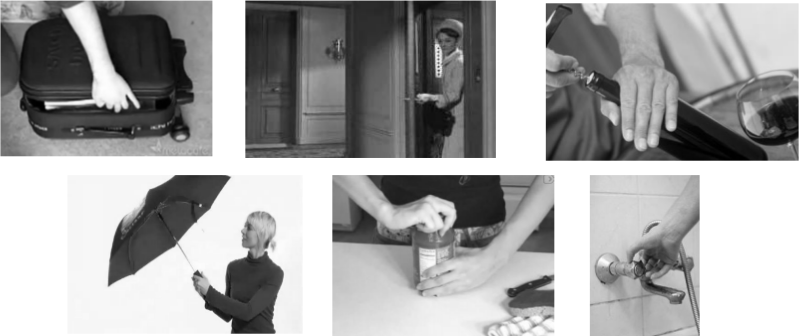
\includegraphics[scale=0.3]{open_example}
  \caption{Παραδείγματα της δράσης «Ανοίγω»}
  \label{fig:open_example}

\end{figure}

Προκειμένου να αντιμετωπιστούν αυτές οι προκλήσεις, έχουν δημιουργηθεί διάφορα σύνολα δεδομένων για ανθρώπινες δράσεις, προκειμένου να αναπτυχθούν
ισχυρά συστήματα αναγνώρισης της ανθρώπινης δράσης και αλγόριθμοι ανίχνευσης.
Τα πρώτα σύνολα δεδομένων περιέλαμβαν έναν δρων χρησιμοποιώντας  μιας στατικής κάμερα πάνω σε ομοιογενή υπόβαθρα.
Παρόλο που αυτά τα σύνολα δεδομένων συνείσφεραν στο να σχεδιάσουμε τους πρώτους αλγορίθμους αναγνώρισης δράσης, δεν ήταν σε θέση να αντιμετωπίσουν αποτελεσματικά τις παραπάνω
προκλήσεις.
Έτσι λοιπόν οδηγηθήκαν στον να δημιουργήσουμε σύνολα δεδομένων που περιέχουν πιο αμφιλεγόμενα βίντεο, όπως το \en Joint-annotated Human Motion Database(JHMDB) (\cite{Kuehne11}) \gr 
και \en UCF-101 (\cite{soomro2012ucf101})\gr. Αυτά τα \en dataset \gr περιλαμβάνουν μόνο ανθρώπινες ενέργειες, η δεύτερη κατηγορία που αναφέρθηκε πιο πριν.

\subsection{\tl{JHMDB Dataset}}
Το σύνολο δεδομένων \en JHMDB (\cite{Jhuang:ICCV:2013}) \gr είναι ένα πλήρες σχολιασμένο σύνολο δεδομένων για ανθρώπινες ενέργειες και ανθρώπινες πόζες. Αποτελείται από 21 κατηγορίες δράσεων
και 928 κλιπ που εξάγονται από την βάση δεδομένων κίνησης του ανθρώπου \en (HMDB51 \cite{Kuehne11})\gr. Αυτό το σύνολο δεδομένων περιέχει κομμένα βίντεο με διάρκεια μεταξύ
15 έως 40 καρέ. Κάθε κλιπ σχολιάζεται για κάθε καρέ χρησιμοποιώντας μια δισδιάστατη στάση και περιέχει μόνο 1 ενέργεια.
Προκειμένου να εκπαιδεύσουμε το μοντέλο μας για τον εντοπισμό των ενεργειών, τροποποιούμε της δισδιάστατες πόζες σε δισδιάσταστα πλαίσια που περιέχουν ολόκληρη τη στάση του δρώντα σε κάθε καρέ.
Υπάρχουν διαθέσιμα 3 διαφορετικά χωρίσματα για να εκπαιδευτεί ένα μοντέλο, τα οποία προτείνουν οι συγγραφείς. Επιλέξαμε το πρώτο  που περιέχει 660
βίντεο στο εκπαιδευτικό σετ και 268 για επικύρωση.

\subsection{\tl{UCF-101 Dataset}}
Το σύνολο δεδομένων \en UCF-101 (\cite{soomro2012ucf101}) \gr περιέχει 13320 βίντεο από 101 κατηγορίες δράσεων.
Από αυτά, παρέχονται χωροχρονικοί  σχολιασμοί για 24 κλάσεις  και 3194 βίντεο. Αυτό σημαίνει ότι σε κάθε βίντεο, υπάρχει ένα \en 2D \gr οριοθετημένο πλαίσιο που περιβάλλει
το άτομο που δρα για κάθε καρέ στο οποίο λαμβάνει χώρα μια δράση.
Διαχωρίζουμε το σύνολο των δεδομένων  σε 2284 βίντεο για εκπαιδευτικό σετ και 910 για σετ επικύρωσης σύμφωνα με το
πρώτο προτεινόμενο διαχωρισμό. Για τα δεδομένα εκπαίδευσης, υπάρχουν βίντεο μέχρι 641 καρέ, ενώ για τα βίντεο επικύρωσης ο μέγιστος αριθμός πλαισίων είναι 900.
Κάθε βίντεο, τόσο για την εκπαίδευση όσο και για την επικύρωση, είναι μη-κομμένο(\en untrimmed\gr), ενώ σε πολλές περιπτώσεις  περισσότερες από 1 ενέργειες πραγματοποιούνται ταυτόχρονα.
Λάβαμε σχολιασμούς από \en \cite{singh2016online} \gr επειδή εκείνουν που μας παρείχαν οι συγγραφείς περιείχαν ορισμένα λάθη.

\section{\enMotivation and Contibutions\gr}
Τα τρέχοντα επιτεύγματα στα δίκτυα αναγνώρισης αντικειμένων και στα \en 3D Convolutional NN για  αναγνώριση ενεργειών μας προκάλεσαν να δοκιμάσουμε
για να τα συνδυάσουμε, προκειμένου να επιτύχουμε τα καλύτερα αποτελέσματα στο πρόβλημα του εντοπισμoύ ανθρώπινης δράσης. Εισάγουμε μια νέα δομή δικτύου εμπνευσμένη από το
\cite{DBLP:journals/corr/HouCS17}, \cite{DBLP:journals/corr/abs-1712-09184}, \cite{Ren:2015:FRT:2969239.2969250} και η υλοποίηση από το  \cite{jjfaster2rcnn}.

Οι συνεισφορές μας είναι οι εξής: 1) Δημιουργούμε ένα νέο \en framework \gr για τον εντοπισμό των ενεργειών που επεκτείνει τον κώδικα που έχει υλοποιηθεί το \en FasterR-CNN,
2) Δημιουργήσαμε ένα δίκτυο για  πρόταση ακολουθιών δυσδιάσταστων κουτιών σε βίντεο κλιπ τα οποία μπορεί να περιέχουν μια δράση, εκμεταλλευόμενοι 
τα χωροχρονικά χαρακτηριστικά που μας παρέχουν οι \en 3D Convolutions\gr, 3) δημιουργούμε έναν αλγόριθμο σύνδεσης για τη σύνδεση των προτεινόμενων ακολουθιών
για να εξάγουμε υποψήφια \en action tubes \gr και 4) προσπαθήσαμε να βρούμε τους καταλληλότερους χάρτες χαρακτηριστικών καθώς και τον κατάλληλο ταξινομητή για να
πραγματοποιήσουμε αποδοτικό \en classification\gr.
\section{\en Thesis structure\gr}
\textbf{NA to ksanadw...}
Η υπόλοιπη διατριβή οργανώνεται ως εξής. Το κεφάλαιο 2 παρέχει μια γενική εισαγωγή στις τεχνικές μηχανικής μάθησης  που χρησιμοποιούνται σήμερα.
Στη συνέχεια, παρουσιάζουμε τα βασικά στοιχεία των συστημάτων αναγνώρισης αντικειμένων παράλληλα με τις συναρτήσεις κόστους  και τις μετρικές που χρησιμοποιήσαμε.
Επίσης, το Κεφάλαιο 2 παρουσιάζει μια σύντομη επισκόπηση της βιβλιογραφίας σχετικά με την αναγνώριση και τον εντοπισμό της ανθρώπινης δράσης.
Το Κεφάλαιο 3 εισάγει το πρώτο βασικό στοιχείο του δικτύου μας, το \en Tube Proposal Network (TPN)\gr, ένα δίκτυο που προτείνει \en Tubes of Interest (ToIs)\gr,
οι οποίες είναι ακολουθίες δυσδιάστατων πλαισίων, που είναι πιθανά να περιέχουν μια εκτελεσθείσα ενέργεια.
Επιπλέον, παρουσιάζονται  όλες τις προτεινόμενες από μας αρχιτεκτονικές για την επίτευξη αυτού του στόχου.
Το κεφάλαιο 4 προτείνει αλγόριθμους για τη σύνδεση των προτεινόμενων \en ToIs \gr από κάθε τμήμα βίντεο και παρουσιάζονται οι επιδόσεις των προτάσεων.
Στο Κεφάλαιο 5 παρουσιάζουμε όλες τις προσεγγίσεις ταξινόμησης που χρησιμοποιήσαμε για τον σχεδιασμό της αρχιτεκτονικής μας και ορισμένα αποτελέσματα ταξινόμησης.
Το Κεφάλαιο 6 χρησιμοποιείται για συμπεράσματα, περίληψη της συμβολής μας μαζί με πιθανές μελλοντικές εργασίες.

% \end{document}
